\documentclass[12pt]{beamer}
%\documentclass[20pt,handout]{beamer}
\usetheme{Darmstadt}
\usepackage{graphicx}
\usepackage[ngerman]{babel}
\usepackage[T1]{fontenc}
\usepackage[utf8]{inputenc}
\usepackage{tikz}
\usepackage[shadow,colorinlistoftodos]{todonotes}
\setbeamertemplate{footline}[frame number]

\newcommand{\cc}[1]{\includegraphics[height=4mm]{img/#1.png}}
\usepackage{ifthen}
\newcommand{\license}[2][]{\\#2\ifthenelse{\equal{#1}{}}{}{\\\scriptsize\url{#1}}}
\usepackage{textcomp}

%%% keine grauen Items in Listen  \setbeamercovered{transparent}

\pgfdeclareimage[height=.6cm]{c3d2logo}{./img/c3d2.pdf}

\pgfdeclarelayer{foreground}
\pgfsetlayers{main,foreground}
\logo{\pgfputat{\pgfxy(-1,0)}{\pgfbox[center,base]{\pgfuseimage{c3d2logo}}}}


\title{Chaos macht Schule}
\author{\small Robert Wartenberg \& Benjamin Partzsch\\\large Chaos Computer Club Dresden}
\date{26.06.2018}

\begin{document}
\maketitle

\section{Einleitung}
\subsection{}

\begin{frame}
	\frametitle{Chaos Computer Club}
	\begin{center}
		
\includegraphics[height=0.2\textheight]{img/chaosknoten.png}
	\end{center}	
	\begin{itemize}
		\item<1-> Verein wurde 1981 gegründet (\url{https://ccc.de})          
		\item<2-> Aktuell mehr als 6000 Mitglieder
		\item<3-> Betreibt u.a. Öffentlichkeitsarbeit und Politikberatung      
		\item<4-> Lokale Erfahrungsaustauschkreise (Erfas) und Chaostreffs
	\end{itemize}
\end{frame}

\begin{frame}
	\frametitle{Chaos Computer Club Dresden}
	\begin{figure}
		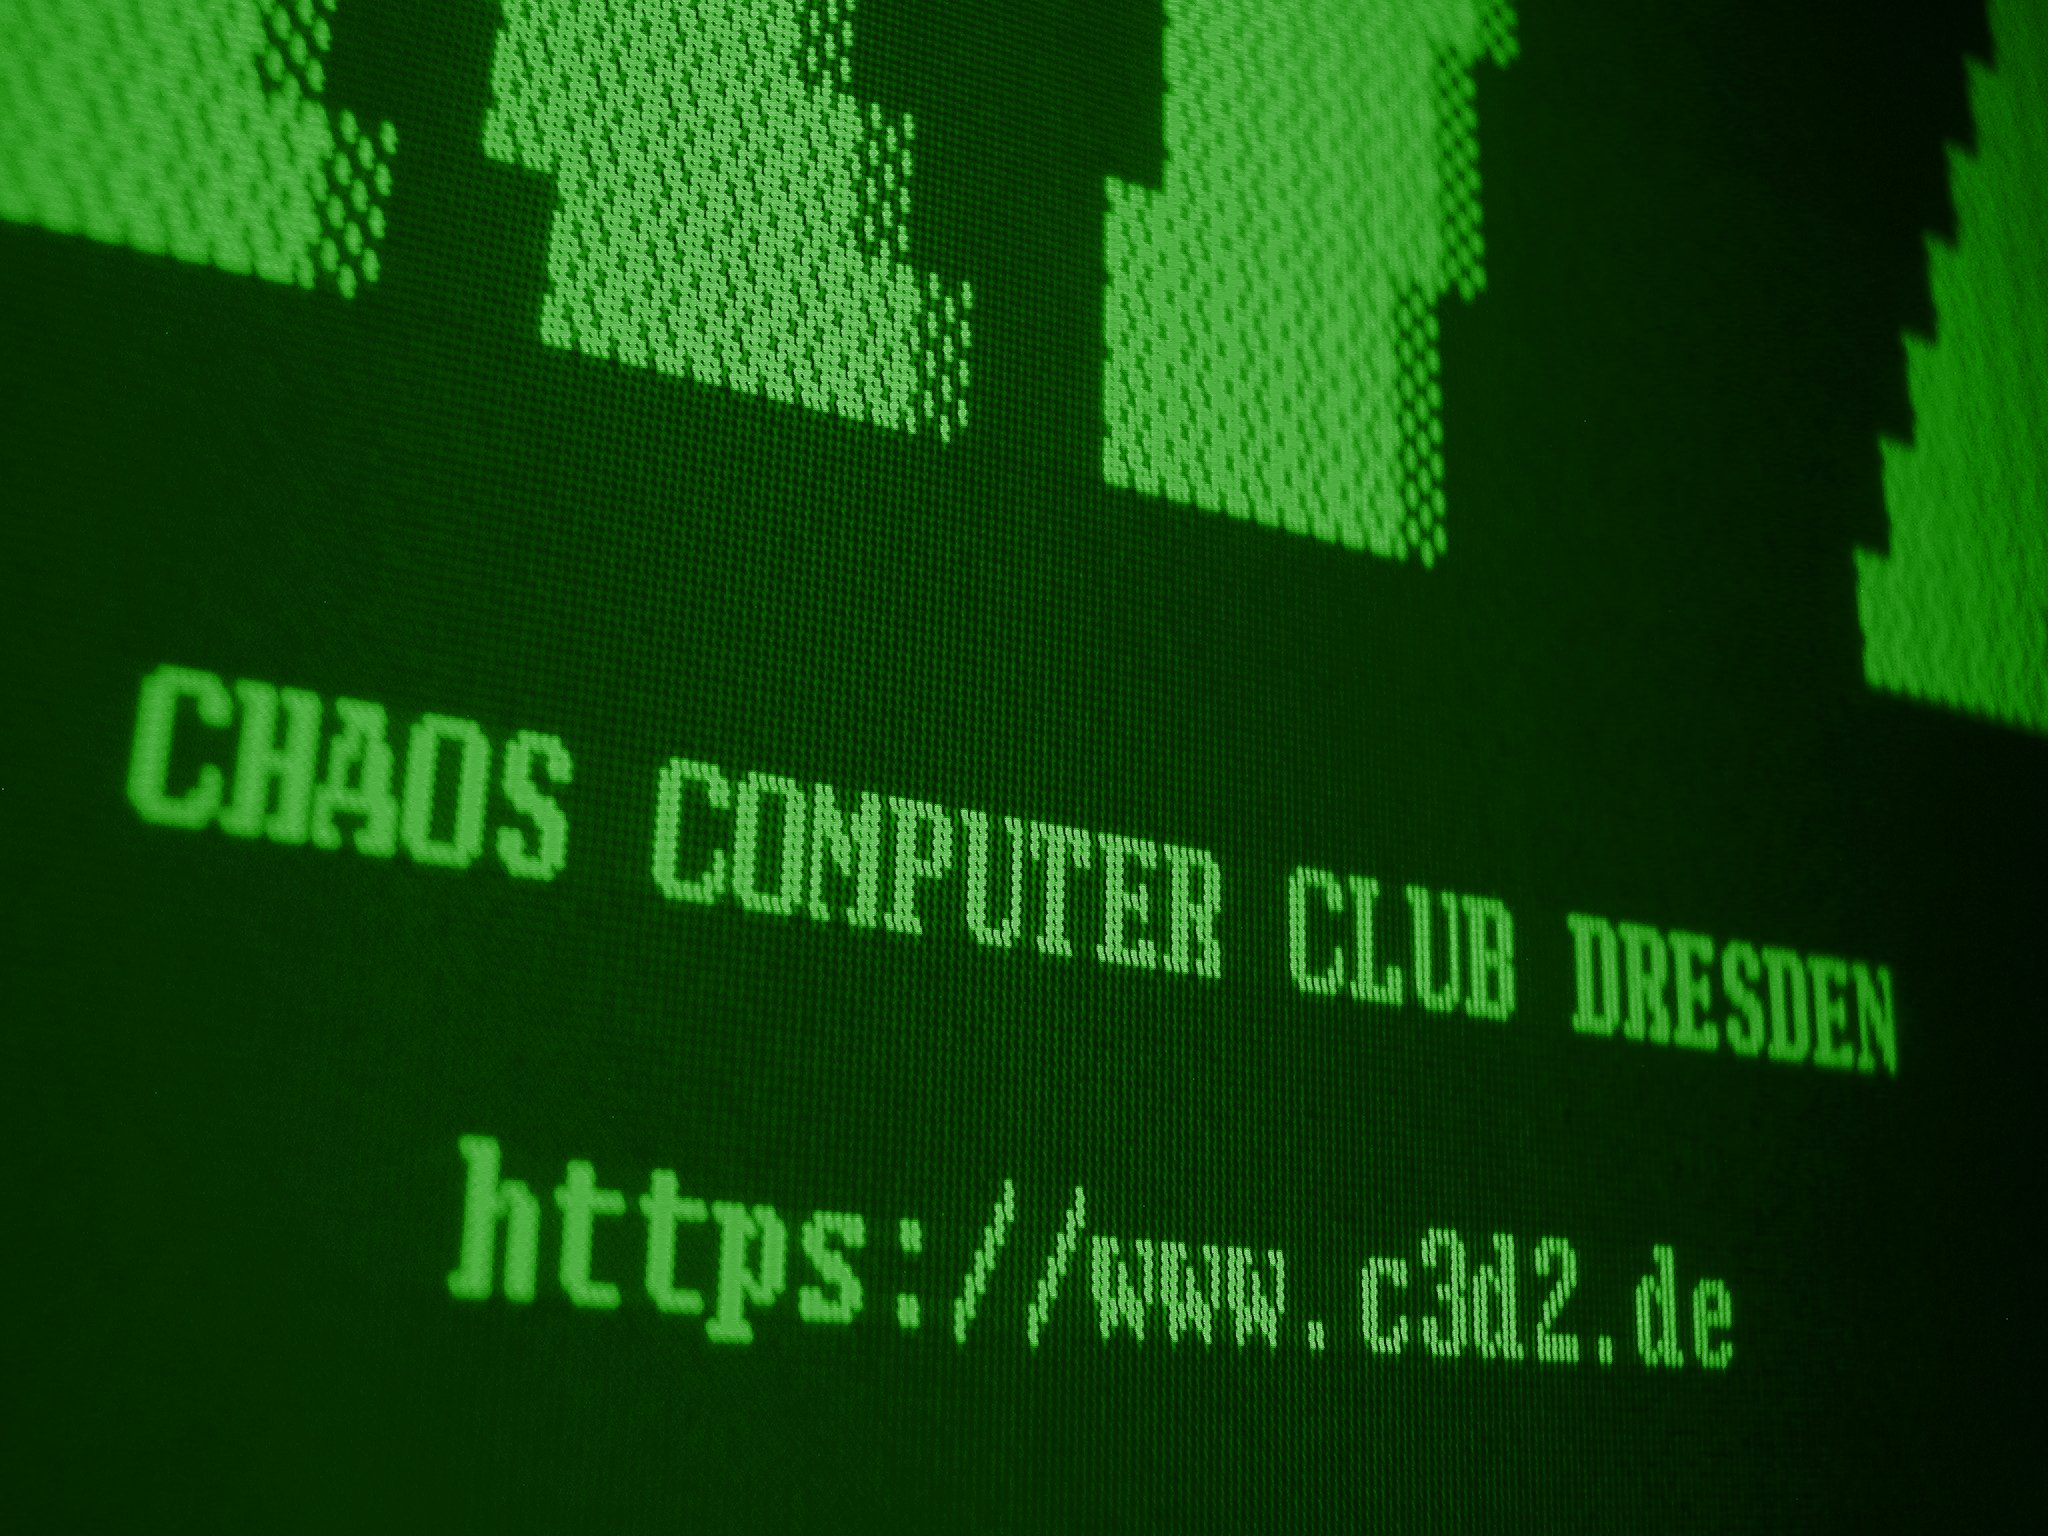
\includegraphics[height=0.7\textheight]{img/c3d2_green.jpg}
    \end{figure}
\end{frame}

\begin{frame}	
	\frametitle{Chaos Computer Club Dresden}
	\begin{center}
		
\includegraphics[height=0.1\textheight]{img/c3d2_logo.png}		

		Erfahrungsaustauschkreis Dresden

		Chaos Computer Club Dresden (\url{https://c3d2.de})

		Radio und Podcasts (\url{https://c3d2.de/radio.html})

		Chaos macht Schule (\url{https://c3d2.de/schule.html})
	\end{center}
\end{frame}	

\begin{frame}	
	\frametitle{Chaos Computer Club Dresden}
	\begin{center}
		
\includegraphics[height=0.1\textheight]{img/c3d2_logo.png}	
		\vspace{1cm}

		Pentaradio und Pentacasts 
		\vspace{1cm}

		\underline{c3d2.de/radio.html}
	\end{center}
\end{frame}	

\begin{frame}	
	\frametitle{Chaos Computer Club Dresden}
	\begin{center}
		
\includegraphics[height=0.3\textheight]{img/cms-text.png}
		\vspace{1cm}

		c3d2.de/schule.html
	\end{center}
\end{frame}	

\end{document}
